\section{GUI}
\label{sec:GUIumsetzung}

Die GUI, der App wird gemäss dem MVC Pattern (Abb. \ref{fig:MVC}) umgesetzt. Der Aufbau von Android unterstützt den Entwickler sich an dieses Pattern zu halten.

\begin{figure}[htbp]
	\centering
	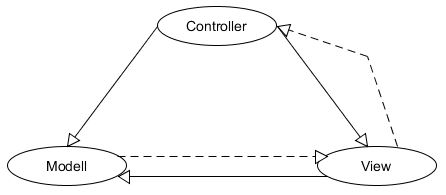
\includegraphics[scale=0.8]{pic/MVC}
	\caption{Modell, View \& Controller Pattern}
	\label{fig:MVC}
\end{figure}

Die Struktur, welche einem von Android vorgegeben wird sieht bei der App wie folgt aus:

\begin{itemize}
	\item Controller - Java Files welche die Funktion beinhalten und die Kommunikation zwischen View und Modell steuern.
	\item View - XML Files welche ausschliesslich das Aussehen der App definieren.
	\item Modell - SQLite Datenbank, welche die Daten für die App beinhaltet.
\end{itemize}

Wie das Pattern umgesetzt wurde anhand einzelner Ausschnitte aus dem Code der App. Auf einen Ausschnitt aus der SQLite Datenbank (dem Modell), wird an dieser Stelle verzichtet. Die Verwendete Datenbank Struktur zeigt die Abbildung \ref{subsec:UebersichtDB}. Sehr schön sieht man das Zusammenspiel zwischen Controller und View an der Zeile 3 \& 4 im Ausschnitt aus dem Button Listener \ref{listener} und der Zeile 2 im Ausschnitt des XML Files \ref{button}.\\

Hier sieht man im Controller eine Switch Verzweigung, welche anhand der übergebenen Button Id (btn\_mng\_author) eine Aktion ausführt. Welche ein neues Layout startet in welchem die Daten aus dem Modell \ref{listItem} angezeigt. 

\lstinputlisting[frame=single,language=java,label=listener,caption=Controller: Button Listener]{code/listenerDB.java}

\lstinputlisting[frame=single,language=xml,label=button,caption=View: Button im XML Layout]{code/button.xml}

\lstinputlisting[frame=single,language=java,label=listItem,caption=Controller: Daten aus Modell in View]{code/listItem.java}

Im Kapitel Anforderung im Abschnitt \ref{sec:GUI} sind noch einige Design Anforderungen dokumentiert, bei welchen ich von einer App mit Bildschirmtabs ausgegangen bin. Dies wurde in einer ersten lauffähigen Alpha Version der App so realisiert. Durch meine dabei gewonnenen Erfahrungen, was die Programmierung und das User Handling der App angeht. Unterstützt von den Ergebnissen einer kleinen Internet Recherche, habe ich alle Design Entscheidungen zu Gunsten einer vertikal scrollenden ScrollView abgeändert. Die Vorteile bei der nun eingesetzten Layout Technik sind.

\begin{itemize}
	\item Modularer und Übersichtlicher Aufbau des Layout.
	\item Skaliert automatisch auf jeden Bildschirm.
	\item Leicht zu erweitern.
	\item Geringerer Aufwand beim Controller der View und damit weniger Fehler anfällig.
\end{itemize} 